\documentclass{sigchi}

% Use this command to override the default ACM copyright statement (e.g. for preprints). 
% Consult the conference website for the camera-ready copyright statement.


% Arabic page numbers for submission. 
% Remove this line to eliminate page numbers for the camera ready copy
%\pagenumbering{arabic}



\usepackage{balance}  % to better equalize the last page
\usepackage{graphics} % for EPS, load graphicx instead
\usepackage{times}    % comment if you want LaTeX's default font
\usepackage{url}      % llt: nicely formatted URLs
\usepackage{graphicx}
\usepackage{caption}
\usepackage{subcaption}
\usepackage{array}
\usepackage{amsmath}
%\usepackage{multirow}

% llt: Define a global style for URLs, rather that the default one
\makeatletter
\def\url@leostyle{%
  \@ifundefined{selectfont}{\def\UrlFont{\sf}}{\def\UrlFont{\small\bf\ttfamily}}}
\makeatother
\urlstyle{leo}


% To make various LaTeX processors do the right thing with page size.
\def\pprw{8.5in}
\def\pprh{11in}
\special{papersize=\pprw,\pprh}
\setlength{\paperwidth}{\pprw}
\setlength{\paperheight}{\pprh}
\setlength{\pdfpagewidth}{\pprw}
\setlength{\pdfpageheight}{\pprh}

% Make sure hyperref comes last of your loaded packages, 
% to give it a fighting chance of not being over-written, 
% since its job is to redefine many LaTeX commands.
%\usepackage[pdftex]{hyperref}
%\hypersetup{
%pdftitle={L@S 2014 Work-in-Progress Format},
%pdfauthor={LaTeX},
%pdfkeywords={SIGCHI, proceedings, archival format},
%bookmarksnumbered,
%pdfstartview={FitH},
%colorlinks,
%citecolor=black,
%filecolor=black,
%linkcolor=black,
%urlcolor=black,
%breaklinks=true,
%}

% create a shortcut to typeset table headings
\newcommand\tabhead[1]{\small\textbf{#1}}

\begin{document}

\title{Making the Grade}
\large

\numberofauthors{2}
\author{
  \alignauthor Casey O'Brien\\
    \email{cmobrien@mit.edu}
\alignauthor Adam Yedidia\\
\email{adamy@mit.edu}
}

\maketitle

\section{Abstract}

\renewcommand*{\arraystretch}{1.5}

\section{Introduction}

Say that you are a student in a large introductory class, like 6.006. Halfway through the semester, you'd really like to know: \textit{How likely is it that I get an A in this class?}

As TA�s for 6.006, we field questions like this all the time. We answer them with a very practiced response, something like: \textit{We cannot make any predictions about final grades before all assignments are graded}. We say this because we do not want to risk making an incorrect prediction and having the student complain at the end of the semester. However, this is basically a blatant lie. In fact, we think that given a student's grades halfway through the semester, we can make a fairly accurate prediction as to what their final grade in the course will be.

Our work will focus on 6.006, \textit{Introduction to Algorithms}. For the past five years, very little about the class has changed. Each semester, there are 9 assignments: 6 problem sets, 2 quizzes, and a final exam. A student's final numerical grade is weighted as 5\% per problem set, 20\% per quiz, and 30\% for the final exam.

There are three different types of problem that we will discuss in this paper.
\begin{enumerate}
\item \textit{Numerical Prediction}: Predict the student's final numerical average.
\item \textit{Letter Prediction}: Predict the student's final letter grade.
\item \textit{Letter Distribution}: Find the probability distribution over a student's final letter grade.
\end{enumerate}

We solved all of these problems at each point throughout the class (i.e., after each assignment was due). This allowed us to see how our predictive power increased as we progressed throughout the semester. As one might expect, we saw the largest decreases in our error rates after each of the quizzes.

To compute the numerical prediction, we used regression. For letter prediction, we tried two different models. The first was to perform regression, and then map numerical scores to letter grades. The second was to use an ordered logit/probit model, which, in turn, solved the letter distribution problem. These models will be discussed in more detail in the coming sections.

\subsection{Data}

We have grade data for six semesters over the past five years. For each student, we have their grade on each assignment, as well as their final letter grade in the class. Within any semester, professors used hard thresholds for letter grade divides. So, if Alice and Bob took 6.006 in the same semester, and Alice has a higher weighted average than Bob, then Alice's letter grade is at least as good as Bob's.

Figure 1 displays information about our dataset. In particular, Figure 1(a) shows the distribution of students over the different majors (note that double majors were counted in both corresponding columns). We can see that almost all students are either courses 6 or 18. Figure 1(b) shows the gender distribution (which is about 2:1 male:female). Figure 1(c) shows the year distribution, where we see that the students are mostly sophomores. Finally, Figure 1(d) shows the distribution over final grades, which is about 41\% A's, 41\% B's, and 18\% C's. Because the number of $D$'s and $F$'s was so sparse, we considered them the same as $C$'s. So, throughout this paper, $C$'s actually refers to $C$'s, $D$'s, and $F$'s. Note that this distribution varies slightly across different semesters.

\begin{figure*}[t!]

\begin{tabular}{c c c}
\multicolumn{3}{ c }{
	\begin{subfigure}[b]{7in}
		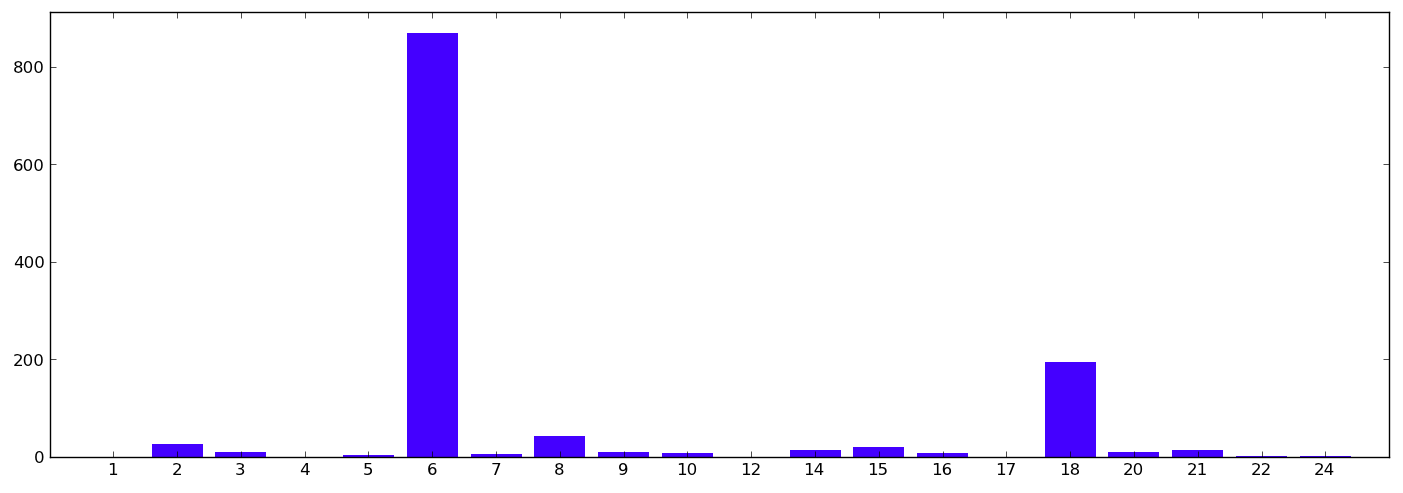
\includegraphics[width=7in]{plots/major.png}
		\caption{CAPTION}
	\end{subfigure}
	}
\\ &&\\
\begin{subfigure}[b]{2.25in}
	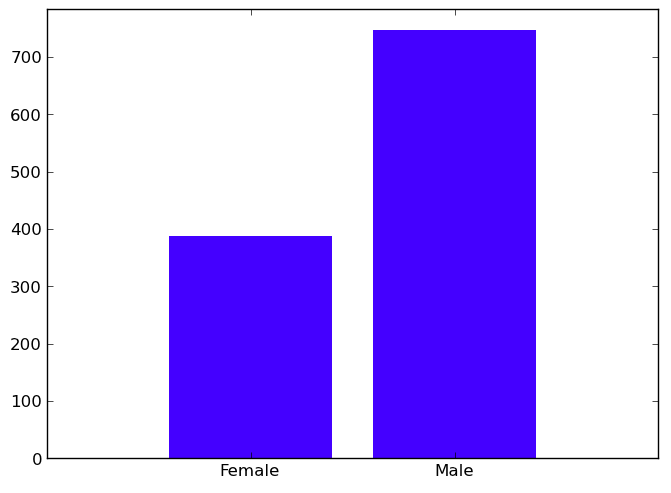
\includegraphics[width=2.25in]{plots/gender.png}
	\caption{CAPTION}
\end{subfigure}
&
\begin{subfigure}[b]{2.25in}
	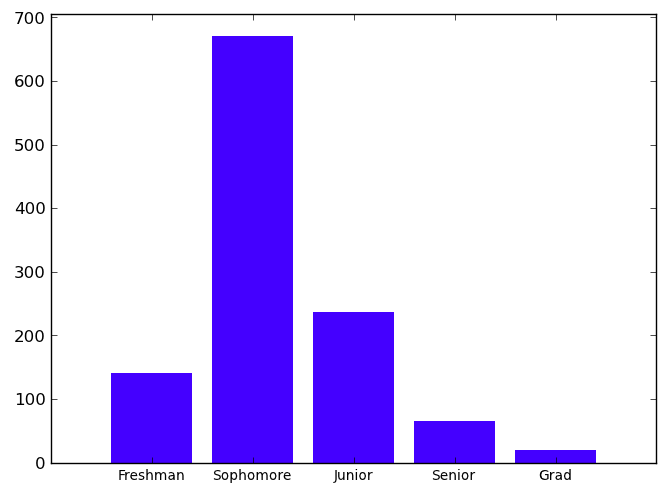
\includegraphics[width=2.25in]{plots/year.png}
	\caption{CAPTION}
\end{subfigure}
&
\begin{subfigure}[b]{2.25in}
	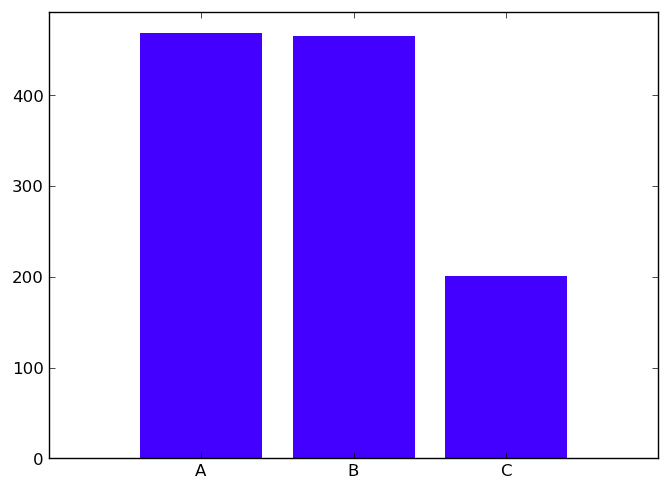
\includegraphics[width=2.25in]{plots/grade.png}
	\caption{CAPTION}
\end{subfigure}
\end{tabular}

\caption{Caption}

\end{figure*}

We would like for our models to be able to predict scores not just in these six semesters, but in future semesters. When this is being used in the future, the test data will consist of students from a single semester, and the goal will be to predict their final grades before we actually know them. As such, we randomly chose a single semester of the six to represent our test data. The test data consists of 197 students. The other five semesters, consisting of 938 students in total, were combined and used as training and validation data.

\subsection{Features}

The first, most obvious features to include were the assignment grades. For each assignment (of the assignments being considered at the time), we included as a feature the difference between the student's score and the mean.  We considered dividing by the standard deviation of the assignment (to get the $z$-score), but we realized this has a key flaw. The weighted sum of the $z$-scores of assignments is not equal to the $z$-score of the weighted sum of raw scores. The result is that when students are sorted by weighted sum of $z$-scores, we no longer have the property that grades obey hard thresholds, as described above.

This is perhaps an interesting issue to consider about the way that we assign grades. Say that Alice scores 20 points below average on a test with a very high variance and 20 points above average on a test with very low variance. Bob, on the other hand, scores 20 points above average on the high variance test and 20 points below average on the low variance test. It seems clear that Alice is performing better in the class, yet by our current grading scheme, both students have the same overall score.

Of course, since all of the semesters for which we have data were not graded using $z$-scores, we do not consider this idea any further here.

In order to make it easier to comprehend the weights resulting from our models, we scaled problem set features to be out of 5 (before subtracting the mean), quiz features out of 20, and the final feature out of 30. The result is that when we compare the weights for say, a problem set and a quiz, we can directly compare the effects of a 1\% change to final score caused by a problem set and a 1\% change to final score caused by a quiz.

Another feature we included is the number of zeros scored on problem sets. For various reasons, some students do not complete certain problem sets throughout the semester. If we are told that a student has an average of 50\% on problem sets after the first two problem sets, we might expect that their future problem set scores be about 50\%. However, if we know that their first problem set score was a 0\% and their second a 100\%, we probably expect their future problem set scores to be much higher than 50\%.

We also included a feature indicating whether the student took the class in the fall or the spring. While we would not expect to see a huge weight corresponding to this feature, it is interesting to see how it affects our predictions.

For the remainder of our features, we included personal data about the students. To obtain this information, we wrote a web scraper to pull the information from the MIT Alumni Database and MIT People. For each student, we recorded their gender, graduation year, and major.

For five students, we were unable to locate their information. For these students, we guessed their gender (with fairly high confidence) based on their names, and assigned their graduation year and major based on the most likely values. We could have used a more sophisticated method here, but because there were so few students in question, it would have been very unlikely to make any difference.

To capture their gender in a feature, we included a binary variable indicating if the student was male. To capture their graduation year, we included a feature containing the undergraduate school year in which they took the class (e.g., 1, 2, 3, or 4). The few graduate students in the class were considered a 5. Finally, to capture major, we included three binary features, indicating if the student was course 6, course 8, or course 18. Students with double majors had both corresponding features on. While we would have liked to consider the binary features for all other majors, the data was too sparse for us to believe we could get a real signal from it.

\subsection{Roadmap}

In the next section, we will discuss our implementation of regression, and how it allowed us to solve the numerical prediction and letter prediction problems. In the following section, we will discuss the ordered logit and probit models, and how they solved the letter prediction and letter distribution problems.

\section{Regression}

\begin{figure*}
\centering
\begin{tabular}{c c}
\begin{subfigure}[b]{3in}
	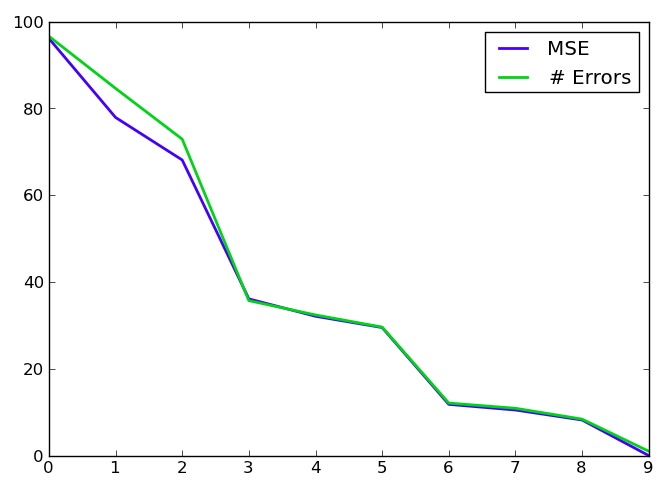
\includegraphics[width=3in]{plots/mse.png}
	\caption{CAPTION}
\end{subfigure}
&
\begin{subfigure}[b]{3in}
	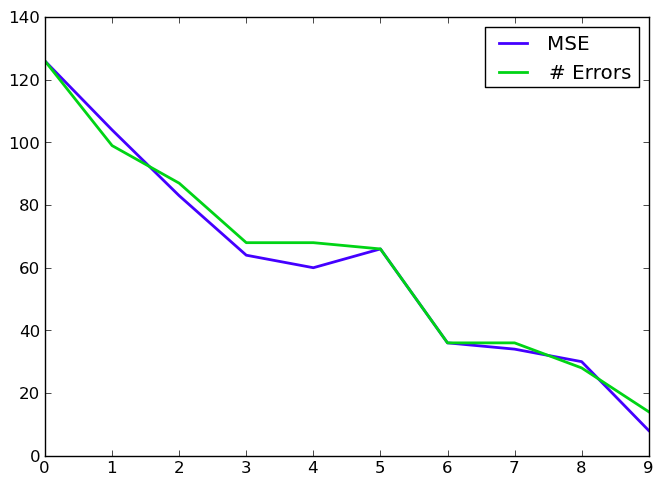
\includegraphics[width=3in]{plots/num_errors.png}
	\caption{CAPTION}
\end{subfigure}
\\
\begin{subfigure}[b]{3in}
	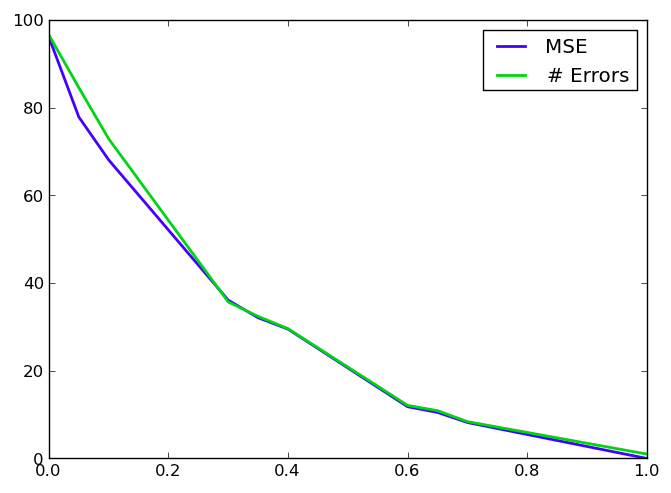
\includegraphics[width=3in]{plots/mse_percentage.png}
	\caption{CAPTION}
\end{subfigure}
&
\begin{subfigure}[b]{3in}
	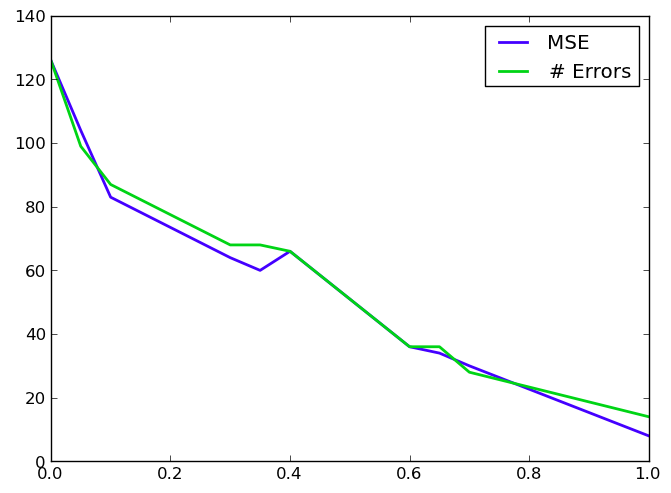
\includegraphics[width=3in]{plots/num_errors_percentage.png}
	\caption{CAPTION}
\end{subfigure}
\end{tabular}
\caption{TEST}
\end{figure*}

\begin{figure}
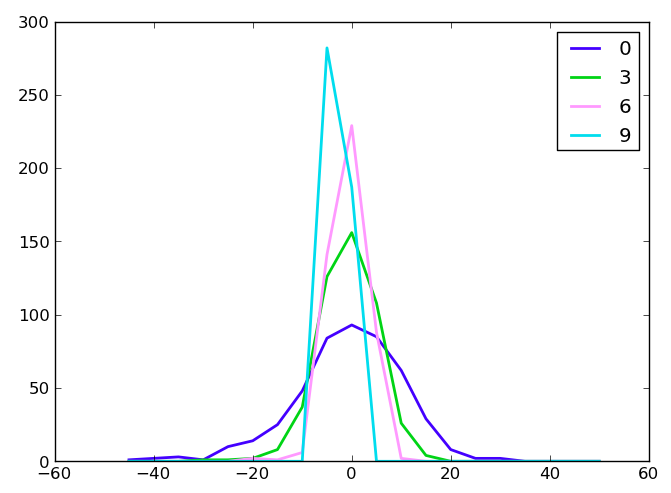
\includegraphics[width = 3in]{plots/gaussian.png}
\caption{CAPTION}
\end{figure}

\begin{figure}
\centering
\begin{tabular}{| c || c | c | c |}
\hline
 &\multicolumn{3}{ c |}{Weights}\\
\hline
Feature & 3 & 6 & 9 \\
\hline
\hline
Problem Set 1 & $$  & $$  & $$ \\
\hline
Problem Set 2 & $$  & $$ & $$ \\
\hline
Quiz 1	       & $$  &  $$ & $$ \\ 
\hline
Problem Set 3 & $-$          & $$ & $$ \\
\hline 
Problem Set 4 & $-$          & $$ & $$  \\
\hline
Quiz 2	       & $-$          & $$ & $$ \\
\hline
Problem Set 5 & $-$          & $-$& $$\\
\hline
Problem Set 6 & $-$          & $-$& $$ \\
\hline
Final		       & $-$          & $-$& $$\\
\hline
Fall		       & $$ & $$ & $$ \\
\hline
Male		       & $$  & $$ & $$ \\
\hline
Year 		       & $$ & $$ & $$\\
\hline
Course 6	       & $$  & $$ & $$ \\
\hline
Course 8	       & $$  & $$ & $$ \\
\hline
Course 18       & $$  & $$ & $$ \\
\hline
\end{tabular}
\caption{THIS SHOULD BE FILLED IN TO HAVE THE WEIGHTS FROM MSE REGRESSION AFTER EACH OF 3, 6, 9 ASSIGNMENTS}
\end{figure}

\section{Ordered Logit/Probit}

This problem seems to lend itself more naturally to classification than to regression. Thus, we decided to model this problem as a classification problem. For this problem, we are no longer interested in predicting student's final numerical scores. Instead, we are only interested in predicting students final letter grade.

Now, given a student's grades and information partway through the semester, we want to predict their final letter grade. This can easily be modeled as a multi-class classification problem. However, the problem is actually more structured than that, because our class values, $A$, $B$, and $C$, have an inherent ordering. Thus, we make use of ordered logit and ordered probit.

These techniques are very similar, so at first we will not differentiate between them. The goal is to map the feature vector, which we will call $x$ for simplicity, to a real number. We will do this by solving for a weight vector $w$, and then mapping $x$ to $x \cdot w$. Then we want to choose cutoffs $\mu_A$ and $\mu_B$ which separate the $A$'s, $B$'s and $C$'s. Once we have solved for $w$, $\mu_A$, and $\mu_B$, we can predict final grades $y$ as follows

\begin{equation} y=
\begin{cases} 
      A &  \mu_A \leq x \cdot w\\
      B & \mu_B \leq x \cdot w < \mu_A \\
      C & x \cdot w < \mu_B 
   \end{cases}.
\end{equation}

Note the lack of $w_0$ term above. We can see that if we chose to include a $w_0$ term, it would simply result in each $\mu$ being offset by $w_0$ as well, leading to an equivalent result. Thus, without limiting our model, we can omit $w_0$.

\subsection{Ordered Probit}

We will first describe the ordered probit model. Say that we assume that a student's final score will be distributed as a Gaussian around their current scores with standard deviation $\sigma$. If we knew the thresholds $\mu_A$ and $\mu_B$, we could calculate the probability that a student received an $A$ in the class as
\[P(y = A) = \Phi \left (\frac{x \cdot w - \mu_A}{\sigma} \right ).\]
Similarly, we have
\[P(y = B) = \Phi \left ( \frac{\mu_A - x \cdot w}{\sigma} \right ) - \Phi \left (\frac{\mu_B - x \cdot w}{\sigma} \right )\]
\[P(y = C) = \Phi \left (\frac{\mu_B - x \cdot w}{\sigma} \right ).\]
From these equations, it is easy to see that if $x \cdot w > \mu_A$, then $P(y = A) > P(y = B) > P(y = C)$. So, whenever we have $x \cdot w > \mu_A$, the maximum likelihood estimate will be $A$. Using similar reasoning for when $x \cdot w < \mu_A$, we can see that equation (1) is simply saying to choose the maximum likelihood estimate.

This works out nicely, but we still need to solve for $w$, $\mu_A$, and $\mu_B$, and now $\sigma$ as well. First, we note that we can set $\sigma = 1$, and it will not restrict our model at all, as we can scale $w$, $\mu_A$, and $\mu_B$ accordingly. So now we have
\[P(y = A) = \Phi \left (x \cdot w - \mu_A \right ).\]
\[P(y = B) = \Phi \left (\mu_A - x \cdot w \right ) - \Phi \left (\mu_B - x \cdot w \right )\]
\[P(y = C) = \Phi \left (\mu_B - x \cdot w \right ).\]
Of all the students that we eventually assign an $A$, we would like to maximize the likelihood that they receive an $A$, and similarly for $B$'s and $C$'s. So, our goal will be to solve the following optimization:
\[\max_{w, \mu_A, \mu_B} L(w, \mu_A, \mu_B),\]
where
\[-log{L(w, \mu_A, \mu_B)} = \prod_{\hat{y}^{(i)} = A} P(y = A)\]
\[\times \prod_{\hat{y}^{(i)} = B} P(y = B)\]
\begin{equation} \times \prod_{\hat{y}^{(i)} = C} P(y = C).\end{equation}
To solve this problem, we instead try to minimize the negative log-likelihood. So, our optimization problem is now
\[\min_{w, \mu_A, \mu_B} -\log{L(w, \mu_A, \mu_B)},\]
where
\[L(w, \mu_A, \mu_B) = -\sum_{\hat{y}^{(i)} = A} \log{P(y = A)}\]
\[- \sum_{\hat{y}^{(i)} = B} \log{P(y = B)}\]
\begin{equation} - \sum_{\hat{y}^{(i)} = C} \log{P(y = C)}.\end{equation}

\subsection{Ordered Logit}

The ordered logit model is very similar to the ordered probit model. The difference is that instead of assuming that future grades are distributed as a Gaussian, we assume that they are distributed according to a logistic distribution. Figure xx shows the differences between the Gaussian distribution and the logistic distribution. A logistic distribution is something like a Gaussian distribution with ``fat tails''.

\begin{figure*}
\centering
\begin{tabular}{c c}
\begin{subfigure}[b]{3in}
	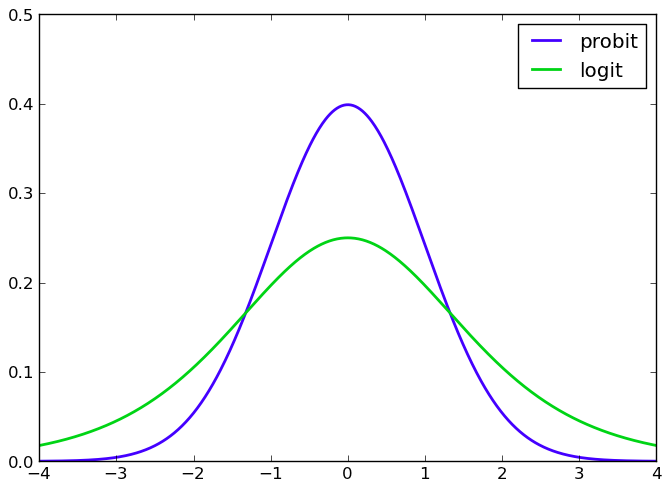
\includegraphics[width=3in]{plots/pdf.png}
	\caption{CAPTION}
\end{subfigure}
&
\begin{subfigure}[b]{3in}
	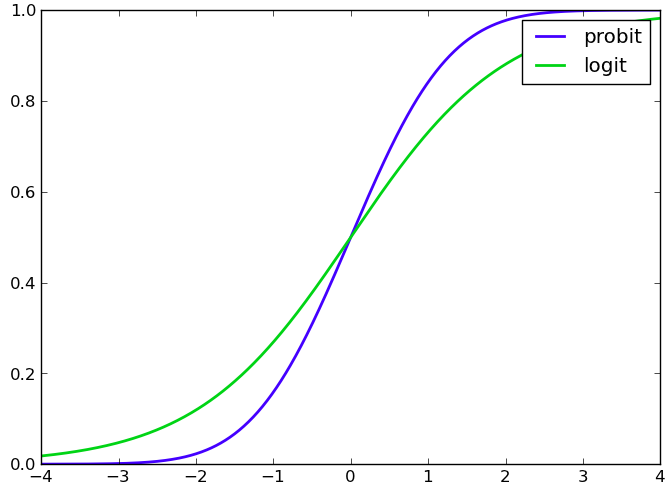
\includegraphics[width=3in]{plots/cdf.png}
	\caption{CAPTION}
\end{subfigure}
\end{tabular}
\caption{TEST}
\end{figure*}

The cumulative distribution function for the logistic distribution is given by
\[F(x) = \frac{1}{1 + e^{-x}}.\]
Thus, to perform ordered logit, we simply need to replace occurrences of $\Phi$ in ordered probit with $F$. So now we have
\[P(y = A) = F \left (x \cdot w - \mu_A \right ).\]
\[P(y = B) = F \left (\mu_A - x \cdot w \right ) - F \left (\mu_B - x \cdot w \right )\]
\[P(y = C) = F \left (\mu_B - x \cdot w \right ).\]
From here, the form of equation xx is unchanged.

\subsection{Choosing a Model}

It's difficult to tell which of the ordered probit or logit models will be more suitable for the data. It depends on knowing how future student grades depend on past student grades. To get a sense for this distribution, we graphed it.

Consider the point in the semester after which we know 3 student grades (two problem sets and a quiz). For each student in the training set, we computed our best guess of their average at that point in the semester (using ridge regression). We then subtracted their final numerical average in the class. The result is the amount that their average changed. Figure xx shows histograms of these values at the beginning of the semester, after 3 assignments, after 6 assignments, and after 9 assignments.

The distributions seem relatively Gaussian, with smaller standard deviations as the semester progresses. This is what we would expect, since later in the semester, much less of the grade is unknown. We also notice that the curves tend to be centered slightly to the left of the origin. 

\subsection{Applying To Our Data}

To solve these optimization problems, we implemented ordered logit and probit in Python, by minimizing the objective functions using \texttt{fmin\_bfgs}.

Next, we applied these models to our data in order to predict student letter grades. As before, we applied both of these models after each assignment throughout the semester. The results were very similar to those described in the Regression section.

\begin{figure}
\centering
\begin{subfigure}[b]{3in}
	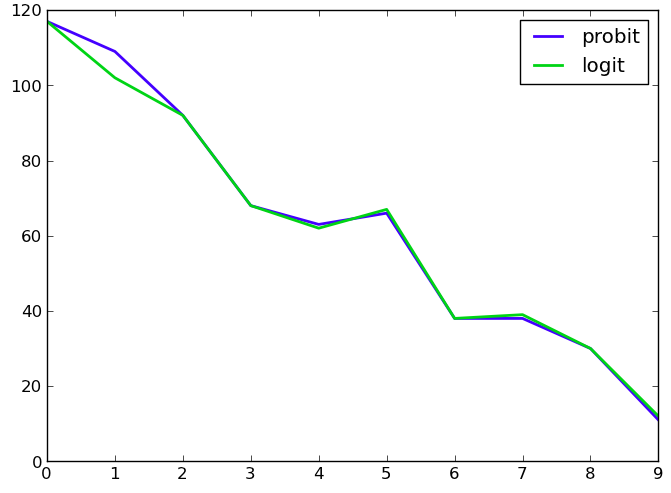
\includegraphics[width=3in]{plots/ordered_num_missed.png}
	\caption{CAPTION}
\end{subfigure}
\begin{subfigure}[b]{3in}
	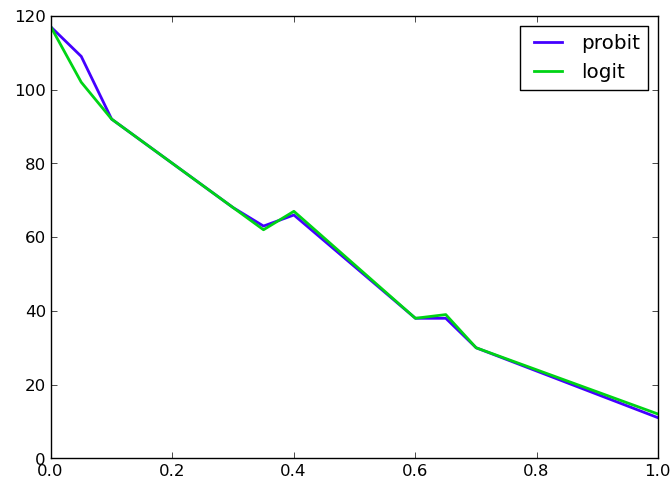
\includegraphics[width=3in]{plots/percentage_num_missed.png}
	\caption{CAPTION}
\end{subfigure}
\caption{Ordered logit/probit number missed}
\end{figure}

Figure xx(a) shows the number of misclassified students as a function of the number of assignments included as features. To properly read this graph, keep in mind the order of assignments:
\[PS1, PS2, Q1, PS2, PS3, Q2, PS4, PS5, F\]
We're not surprised to see that we see the largest drops in number of misclassified students after the 3rd, 6th, and 9th assignments, as these assignments make up the largest proportions of student grades.

This graph is slightly misleading, as it should obviously be the case that the assignments which make up the largest percentages of their grades give us the most information. In Figure xx(b), we see the same curves, but plotted against the percentage of the final grade which had been determined after that assignment.

After the first quiz, students have only completed 30\% of their final weighted grade. Even at this point in the semester, we are able to classify student's final grades with 65\% accuracy. After the second quiz, when 60\% of the final grade is determined, we are able to classify student grades with 81\% accuracy. After the final, when 100\% of the final grade is determined, we classify student grades with 94\% accuracy.

We notice that the amount that our error decreases is not quite linear in the number of percentage points which we include in the features. This implies that as know more about student grades, each additional percentage point tells us less information than the previous. It is also interesting to note that problem set percentage points improve our predictions by just as much as quiz percentage points. In other words, the amount by which our error decreases after a problem set appears to be about one-quarter the amount by which our error decreases after a quiz.

Note that the most common grade among the training and validation data was a $B$. Thus, we can compare these results to the case where we assign $B$'s to all students in the class. This would result in a test error of 122 (corresponding to a 37.8\% accuracy rate), which is slightly worse than that achieved by ordered logit/probit, even when no assignments are considered. Thus, using just personal information about the students, we are able to do better than the trivial algorithm.


It is somewhat disappointing that we are not able to determine final grades with 100\% accuracy, even when all of their scores are completely determined. The reason for this is variation among thresholds from different professors. If professors observed strict proportions of $A$'s, $B$'s, and $C$'s, we could easily predict grades with 100\% accuracy after the final. Sadly, MIT does not allow such grading policies.

\subsubsection{Feature Weights}

To see how important the models consider the various features, let us look at the weights that they produce for each feature at various points throughout the semester.

Figure 3 shows the weights assigned to each feature after 3, 6, and 9 assignments (note that these mark the points after each quiz/final) for ordered probit. The weights for ordered logit are very similar, so we do not display them here. We can observe some general trends from looking at these weights. First, the assignment scores tend to carry a lot more weight than the personal information, which is expected.

The weights of all the assignments tend to be very similar. Recall that the values of the features already take into account the fact that different assignments have different weights in their final grades, so we expect these weights to be roughly equal.

We do see some variety among the weights, although we believe this is because there is some noise introduced by the fact that these assignments had different variances (and the variances differed slightly among years). For example, most students perform very well on problem set 1. Thus, a students score on problem set 1 does not give us much information about their final grade. We believe this is why we tend to see a much lower weight on the first problem set. 

\begin{figure}
\centering
\begin{tabular}{| c || c | c | c |}
\hline
 &\multicolumn{3}{ c |}{Weights}\\
\hline
Feature & 3 & 6 & 9 \\
\hline
\hline
Problem Set 1 & $0.173$  & $0.116$  & $0.361$ \\
\hline
Problem Set 2 & $0.449$  & $0.226$ & $0.463$ \\
\hline
Quiz 1	       & $0.489$  &  $0.454$ & $0.487$ \\ 
\hline
Problem Set 3 & $-$          & $0.532$ & $0.442$ \\
\hline 
Problem Set 4 & $-$          & $0.391$ & $0.302$  \\
\hline
Quiz 2	       & $-$          & $0.381$ & $0.346$ \\
\hline
Problem Set 5 & $-$          & $-$& $0.617$\\
\hline
Problem Set 6 & $-$          & $-$& $0.284$ \\
\hline
Final		       & $-$          & $-$& $0.503$\\
\hline
Fall		       & $-0.083$ & $-0.195$ & $-0.227$ \\
\hline
Male		       & $0.065$  & $0.004$ & $0.050$ \\
\hline
Year 		       & $-0.096$ & $0.001$ & $0.012$\\
\hline
Course 6	       & $0.028$  & $0.192$ & $0.488$ \\
\hline
Course 8	       & $0.026$  & $0.050$ & $-0.005$ \\
\hline
Course 18       & $0.337$  & $0.098$ & $0.152$ \\
\hline
\end{tabular}
\caption{TEST}
\end{figure}


\subsubsection{Grade Distributions}

Next, we move on to focus on the grade distribution problem. Note that when we solved the ordered logit/probit, we already solved the grade distribution problem. To solve the grade prediction problem, we simply chose the most likely estimate. However, this is just throwing away additional information.

Consider a student who comes to you, their TA, after quiz 1, wanting to know what their final grade will be. If you, the TA, predict they will get an $A$, and then they end up with a $B$, they will probably be very unhappy with you at the end of the semester. Instead, if you tell them they have a 52\% chance of getting an $A$ and a 48\% change of getting a $B$, they will probably by much less angry come the end of the semester.

With this in mind, perhaps finding the number of misclassified students is not the correct function to focus on. In fact, this was not the function that we minimized when we solved the ordered logit/probit problem. Recall that our goal was to minimize the negative log likelihood.

While we chose to minimize the negative log likelihood (as opposed to just maximizing the likelihood), the value of this function has some interesting properties. In some sense, we can think of it as a penalty function for an assignment of distributions. A lower penalty corresponds to a better distribution. 

We notice that if we assign a student a 0\% chance of receiving a grade that they eventually receive, then our penalty is $\infty$. This is desirable, because if we are ever so sure that a student has a 0\% chance of receiving a grade, and we end up being wrong, our predictor is clearly doing a very poor job (note that our algorithm will never assign a probability of 0\%, just arbitrarily small probabilities).

We also notice that if we guess their grade correctly with 100\% certainly, we suffer no penalty. This also seems appropriate. If we are entirely sure of a student's final grade, then we should not be penalized for our guess.

Figure xx shows the values of the minimum values of the negative log likelihoods after each assignment is due, for both ordered logit and probit. Interestingly, they produce nearly identical results. This is good news, because it means that the distributional assumptions are not driving the result. As in Figure xx, we show both the curves as a function of the number of assignments completed (in Figure xx(a)), and as a function of percentage of the grade completed (in Figure xx(b)). 

In Figure xx(b), we also observe that the value of the slope decreases slightly as we determine more of their final grades. Again, this points to the fact that as we move through the semester, each additional determined percentage point tells us less than the previous.

%As a result, we introduce a scoring rule for a set of distributions. Let $p^{(i)}$ represent the probability we assigned to student $i$ receiving their actual grade, $y^{(i)}$. So, for example, if we assigned student $i$ a 40\% chance of receiving an A, and the student eventually received an $A$, we would have $p^{(i)} = 0.4$.

%The scoring rule will assign a penalty to each each prediction that we make. If our prediction is bad, we will have a large penalty. The scoring rule we will use here is the logarithmic scoring rule [1], which assigns each prediction a score of $\log(p^{(i)})$. This is a common strictly proper scoring rule, which has a few desirable properties.

%First, we notice that if we assign a student a 0\% chance of receiving a grade that they eventually receive, then our punishment is $-\infty$. This is desirable, because if we are ever so sure that a student has a 0\% chance of receiving a grade, and we end up being wrong, our predictor is clearly doing a very poor job.

%We also notice that if we guess their grade correctly with 100\% certainly, we suffer no penalty. This also seems appropriate. If we are entirely sure of a student's final grade, then we should not be penalized for our guess.

%When we perform ordered logit/probit on our data set, we want to compute the score of the entire test set. To do so, we compute
%\[\sum_{i} \log \left (p^{(i)} \right).\]
%We note that this value is between $-\infty$ and $0$, and will be more negative for a distribution which lacks confidence and/or makes a lot of bad predictions.

%Now, we apply this to the distributions computed by both ordered logit and probit. Interestingly, they produce nearly identical results. This is good news, because it means that the distributional assumptions are not driving the result. Figure xx shows the negative of the score for each of the ordered logit and probit models. We chose to plot the negative because it seems to produce a more intuitive graph.

\begin{figure}
\centering
\begin{subfigure}[b]{3in}
	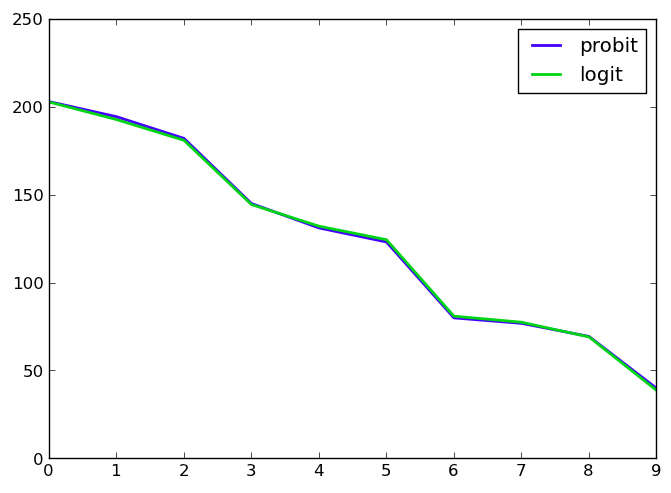
\includegraphics[width=3in]{plots/ordered_score.png}
	\caption{CAPTION}
\end{subfigure}
\begin{subfigure}[b]{3in}
	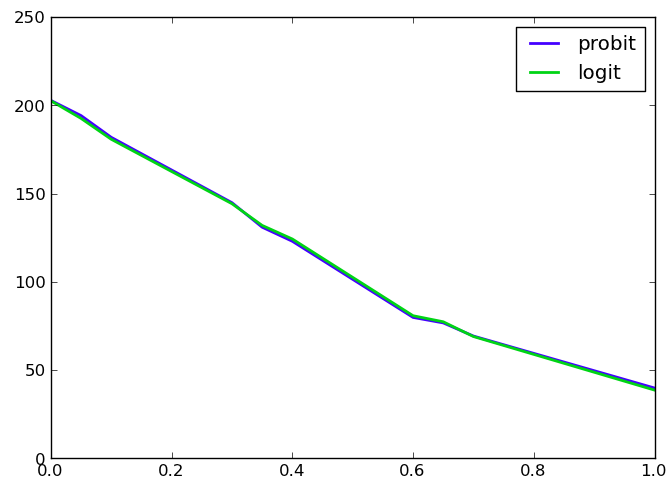
\includegraphics[width=3in]{plots/percentage_score.png}
	\caption{CAPTION}
\end{subfigure}
\caption{Ordered logit/probit number missed}
\end{figure}

In our training and validation data, we observe 41.0\% $A$'s, 41.7\% $B$'s, and 17.3\% $C$'s. We could trivially assign each student in the test set this probability distribution. In the test set, there are 83 $A$'s, 74 $B$'s, and 39 $C$'s. Using this assignment, the negative log likelihood would be
\[- 83 \cdot \log(0.410) - 74 \cdot \log(0.417) - 39 \cdot \log(0.173)\]
\[ = 207.15\]
Again, we notice that even with no assignments included in the features, our ordered logit/probit is able to do slightly better than the trivial solution.

%As before, we observe the greatest changes after assignments 3, 6, and 9, corresponding to the two quizzes and the final. 

%Another interesting idea to consider when discussing distributions is the idea of allowing us to declare uncertainty. Say that we were able to predict one of the grades $A$, $B$, or $C$, or declare that we were uncertain about a grade. We can designate a threshold $T$ such that if the most likely estimate has probability less than $T$, then we conclude that we are uncertain about a students final grade.

%There is a trade-off here. As we raise the threshold, we will decrease the number of incorrectly guessed probabilities, and

%In this situation, we are finally able to see a difference between when we use the ordered logit or the ordered probit model. In the ordered logit model, we think events far from the mean are more likely. Thus, in the logit model, it is harder to become sure of something. Because we are less sure both about the students we predict correctly and the students we predict incorrectly, the total score ends up being almost the same as that of ordered probit.

%In this new scenario, the ordered logit model will be more likely to classify a point as unknown. These results are displayed graphically in Figure xx. 

\begin{figure*}
\centering
\begin{tabular}{c c}
\begin{subfigure}[b]{3in}
	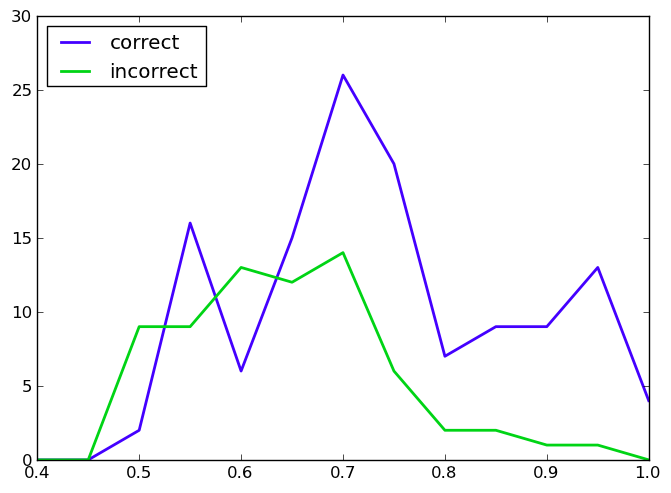
\includegraphics[width=3in]{plots/probit3dist.png}
	\caption{CAPTION}
\end{subfigure}
&
\begin{subfigure}[b]{3in}
	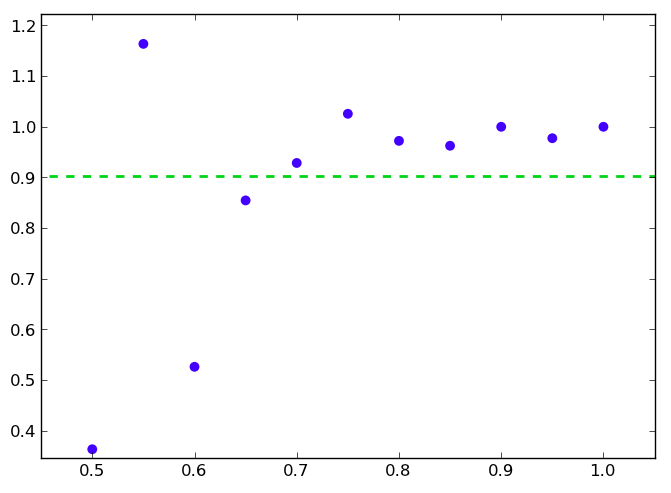
\includegraphics[width=3in]{plots/1pro3.png}
	\caption{CAPTION}
\end{subfigure}
\\
\begin{subfigure}[b]{3in}
	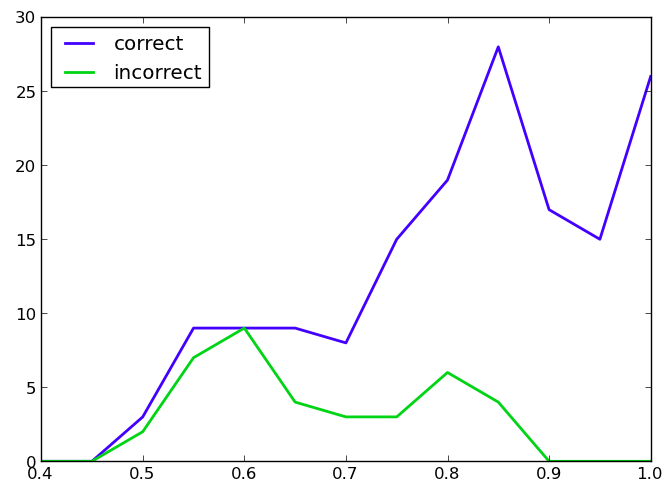
\includegraphics[width=3in]{plots/probit6dist.png}
	\caption{CAPTION}
\end{subfigure}
&
\begin{subfigure}[b]{3in}
	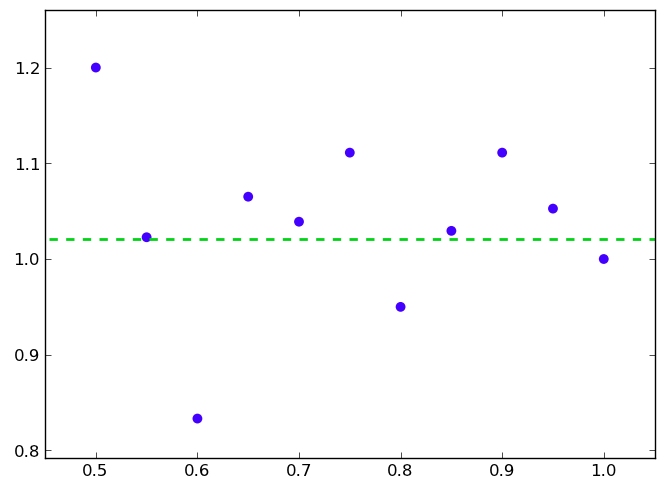
\includegraphics[width=3in]{plots/1pro6.png}
	\caption{CAPTION}
\end{subfigure}
\\
\begin{subfigure}[b]{3in}
	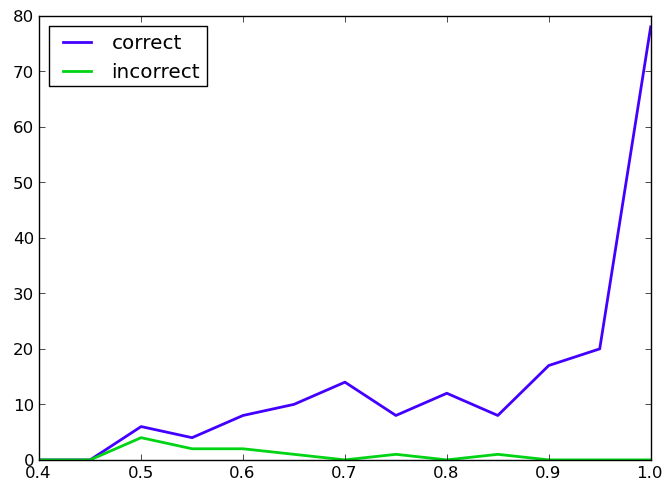
\includegraphics[width=3in]{plots/probit9dist.png}
	\caption{CAPTION}
\end{subfigure}
&
\begin{subfigure}[b]{3in}
	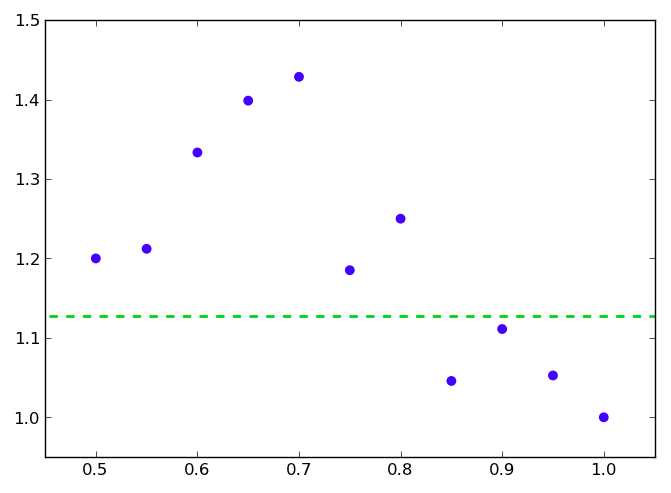
\includegraphics[width=3in]{plots/1pro9.png}
	\caption{CAPTION}
\end{subfigure}
\end{tabular}
\caption{TEST}
\end{figure*}

\subsubsection{Understanding the Distributions}

It is also interesting to try to get a feel for how these distributions actually looked. To start, let's consider a few test points, and look at their distributions after the first quiz (these are not real students). Consider three students taking 6.006 in the spring. Ben is a senior in course 6. He scored exactly average on the first two problem sets and first quiz. Jeremy is a freshman in course 6, and also scored average on the first two problem sets and first quiz. Paul is also a freshman in course 6. He scored average on the first two problem sets, but 10\% above average on the first quiz.

Figure xx shows the distribution returned by ordered probit (ordered logit has the same trends and very similar results, so we do not display it here). It may be surprising that age plays such a large role here. However, in the training data, we see that 66.2\% of freshman received A's in the class, while only 32.5\% of seniors did. With this in mind, their differences are not too surprising.


\begin{figure}
\centering
\begin{tabular}{|c | c | c | c |}
\hline
Student & $P(y = A)$ & $P(y = B)$ & $P(y = C)$\\
\hline
Ben & $28.1\%$ & $66.9\%$ & $5.0\%$\\
\hline
Jeremy & $38.6\%$ & $58.7\%$ & $2.7\%$\\
\hline
Paul & $57.9\%$ & $41.4\%$ & $0.07\%$\\
\hline
\end{tabular}
\caption{CAPTION}
\end{figure}



Let us take a more general look at the distributions in the test set. We attempt to represent this information graphically in Figure xx. Recall that for each student, we found the maximum likelihood estimate, and then classified their grade according to that.

Focus on Figure xx(a). Consider all the students who we were able to correctly guess their final grade. Lets focus on the values of the probabilities we assigned to their maximum likelihood estimates. The blue line represents a histogram of these values, bucketed to intervals of 5\% (we did not display the histogram in the bar form so that we could show multiple on the same graph). The green line is a similar histogram for students that we were not able to correctly guess their final grade.

The charts in the left column were all generated using distributions from the ordered logit model, and the charts in the right column were all generated using distributions from the ordered probit model. The rows correspond to different points throughout the semester. The first row is after three assignments (two pests and a quiz), the second row is after six assignments (four pests and two quizzes), and the last row is after all nine assignments.


%, we display the proportion of students who had an maximum likelihood of at least a certain value, for students classified correctly and incorrectly, for both the ordered logit and probit models. The different subfigures represent different points throughout the semester. 

There are a few interesting trends we can see from these graphs. First, we look at how the values of the maximum likelihoods differed for those students that we were able to classify correctly, and those who we classified incorrectly. We can see that both the ordered logit and probit consistently tended to place higher probabilities on the students that they were ultimately able to classify correctly. This is comforting. It means that the models, in general, claimed to be less sure about the ones which they got wrong than the ones they got right.

We're also interested in how the maximum likelihoods differed between the ordered logit and probit models. This actually is not especially apparent in these graphs, although it becomes much more obvious in the cumulative versions of these graphs (which we do not display here). In general, the ordered logit models tends to be more sure than the ordered probit model (corresponding to higher values for the maximum likelihood).

Finally, we can see how the maximum likelihoods changes throughout the semester. The general trend we see is that as time passes, the models assign higher probabilities to the ones they ultimately classified as correct, and lower probabilities to the ones they ultimately classified as incorrect. This is expected behavior. As the model receives more information, it is given more reason to be sure of the answers that it has classified correctly, and more reason to be unsure of the ones classified incorrectly.

\section{Distributions with Regression}


\begin{figure*}
\centering
\begin{tabular}{c c}
\begin{subfigure}[b]{3in}
	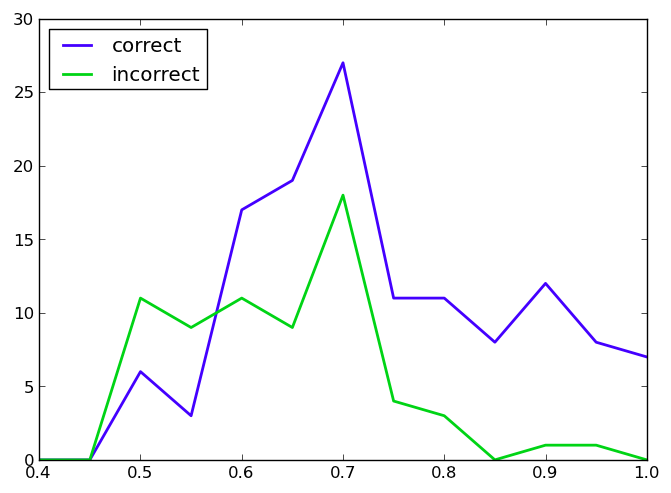
\includegraphics[width=3in]{plots/adam3dist.png}
	\caption{CAPTION}
\end{subfigure}
&
\begin{subfigure}[b]{3in}
	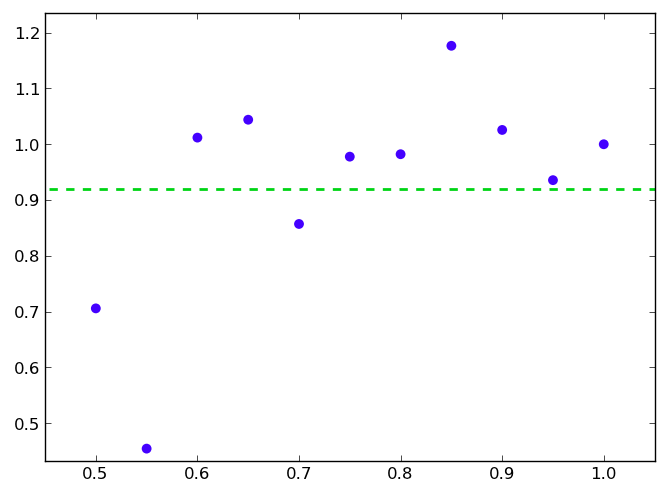
\includegraphics[width=3in]{plots/1adam3.png}
	\caption{CAPTION}
\end{subfigure}
\\
\begin{subfigure}[b]{3in}
	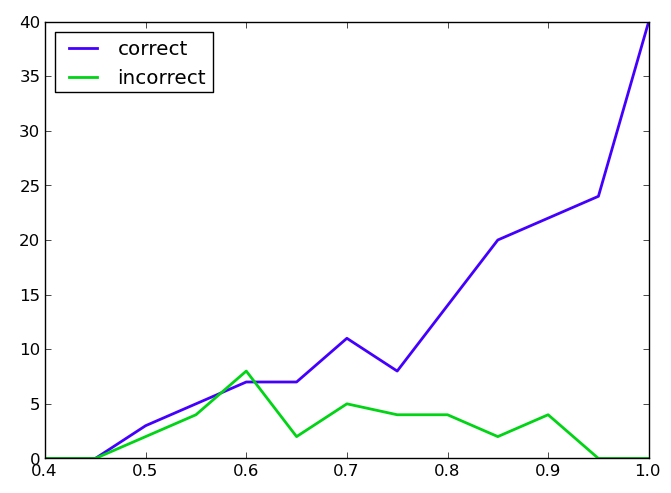
\includegraphics[width=3in]{plots/adam6dist.png}
	\caption{CAPTION}
\end{subfigure}
&
\begin{subfigure}[b]{3in}
	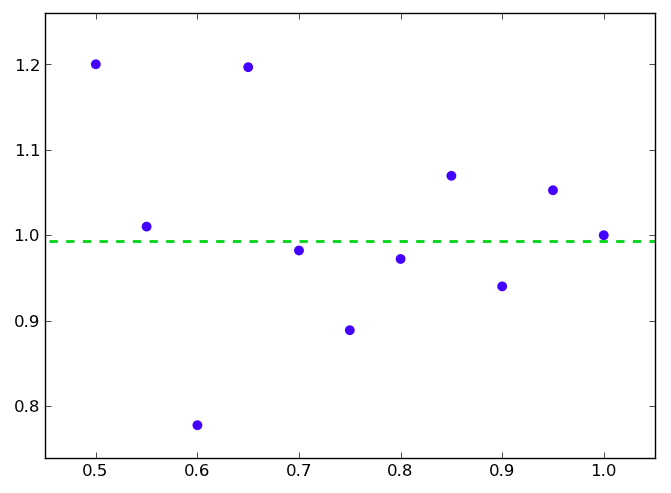
\includegraphics[width=3in]{plots/1adam6.png}
	\caption{CAPTION}
\end{subfigure}
\\
\begin{subfigure}[b]{3in}
	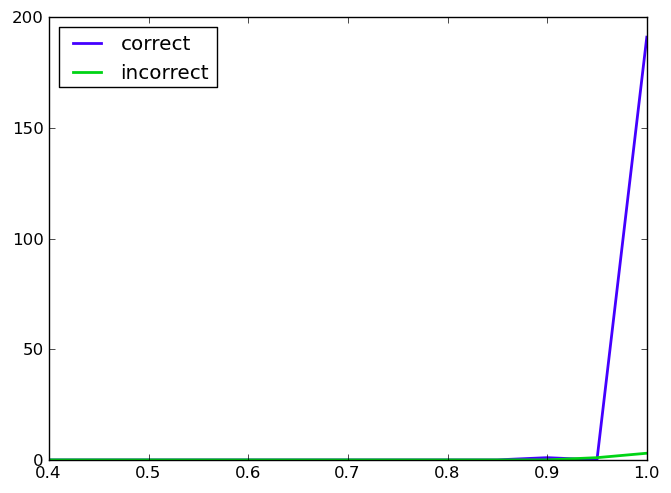
\includegraphics[width=3in]{plots/adam9dist.png}
	\caption{CAPTION}
\end{subfigure}
&
\begin{subfigure}[b]{3in}
	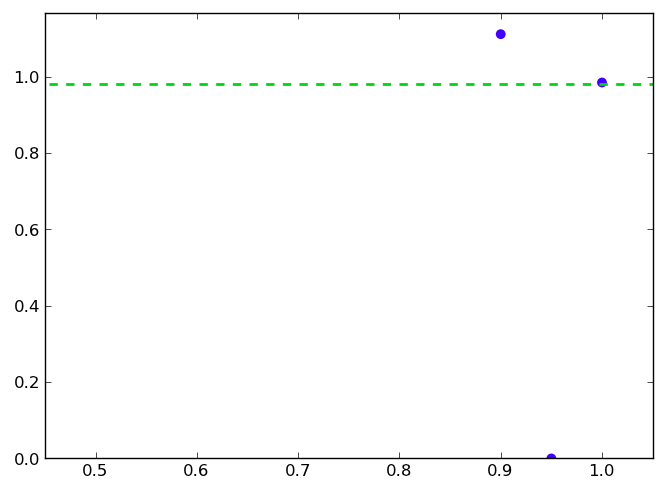
\includegraphics[width=3in]{plots/1adam9.png}
	\caption{CAPTION}
\end{subfigure}
\end{tabular}
\caption{TEST}
\end{figure*}

\section{Discussion}

\end{document}